\chapter{Matériels et Méthodes}

Méthode CRISP\cite{crisp}

Évaluation de nos modèles \cite{plasticc_team_2019_2539456}

\section{Compréhension du problème}

Dans cette section nous .....
Nous passerons en revue les objectifs de ce projets en termes .... et ....
Enfin nous proposerons un plan de projet.


\section{Compréhension des données}
La compréhension des données est l’une des étapes les plus importantes pour la réalisation d’un projet data mining elle vise à déterminer précisément les données à analyser, à identifier la qualité des données disponibles et à faire le lien entre les données
et leur signification d’un point de vue métier. La Data Science étant basée sur les données seules, les problèmes métiers relatifs à des données existantes, qu’elles soient internes ou externes, peuvent ainsi être résolus par la Data Science. Les données sont mises à
disposition sur kaggle-plasticc-challenge.

\subsection{présentation des données}
Pour la réalisation du projet l’équipe plasticc-challenge à mit à notre disposition deux table de données qui sont partagées en données de Test et données d’entraînements .
\newline
\newline
\textbf{[training/test]-set-metadata :} Informations sur les objets qui ne changent pas dans le temps, comme les coordonnées de l’objet, voici les attributs de cette table.
\begin{itemize}
    \item \textbf{object-id :} identifiant d’objet unique de type Integer.
    \item \textbf{ra :} désigne l’ascension droite d’un objet, qui est une coordonnée ciel : co-longitude en degrés de type Float qui est calculé à partir de la différence de la latitude et 90°.
    \item \textbf{ decl:} la déclinaison d’un objet dans le ciel ou co-latitude en degrés de type Float.
    \item \textbf{ gal-l :} désigne la longitude galactique en degrés de type Float.
    \item \textbf{gal-b : }désigne la latitude galactique d’un objet en degrés de type Float.
    \item \textbf{ ddf :} Un drapeau pour identifier l’objet comme provenant de la zone de levé DDF (avec la valeur DDF = 1 pour le DDF, DDF = 0pour le levé WFD). si les champs DDF sont contenus dans la totalité de la zone d’enquête de la DCE, les incertitudes des flux DDF sont bien moindres de type Booléen.
    \item \textbf{ hostgal-specz : }le redshift spectroscopique de la source (décalage vers le rouge). Il s’agit d’une mesure extrêmement précise du décalage vers le rouge, disponible pour l’ensemble d’entraînement et une petite fraction de l’ensemble d’essai de type Float, les objet qui sont de redshift=ൡ sont galactiques.
    \item \textbf{hostgal-photoz :} Redshift photométrique de la galaxie hôte de la source astronomique. Bien que cela soit censé être un proxy pour hostgal-specz, il peut exister de grandes différences entre les deux et doit être considéré comme une version beaucoup moins précise de hostgal-specz cet attribut est de type Float.
    \item \textbf{hostgal-photoz-err :} L’incertitude sur hostgal-photoz d’après les projections de l’enquête LSST cet attribut est de type Float.
    \item \textbf{distmod :} La distance à la source calculée à partir de hostgal-photoz et en utilisant la relativité générale qui est une théorie relativiste de la gravitation, c’est-à-dire qu’elle décrit l’influence sur le mouvement des astres de la présence de matière et, plus généralement d’énergie, en tenant compte des principes de la relativité restreinte, cet attribut est de type Float.
    \item\textbf{mwebv :} MW E (BV). cette «extinction» de la lumière est une propriété de la poussière de la voie lactée (MW) le long de la ligne de mire de la source astronomique et est donc fonction des coordonnées du ciel de la source ra, décl. Ceci est utilisé pour déterminer une gradation et un redimensionnement de la lumière provenant de sources astronomiques dépendant de la bande passante, de type FLOAT.
    \item\textbf{}
    \item\textbf{}
    \item\textbf{}
\end{itemize}



















\section{Préparation des données}\label{sec:data_preparation}


\section{Modélisation}

Les étapes précédentes nous ont permis de construire, à partir des données initiales, un data-set qui n'a plus de données manquantes et qui peut être utilisé pour entraîner des modèlprédictions. Nous avons basé notre modélisation sur deux principales classes de modèles:
\begin{itemize}
    \item \textbf{Les modèles basés sur les caractéristiques :} Il s'agit ici de modèles qui se basent sur les méta données et sur les caractéristiques telles que la moyenne, les quartiles, la valeur maximale, la valeur minimale et bien d'autres pour faire les prédictions. Ces modèles supposent que les séries d'une même classes ont des caractéristiques similaires tandis que les séries de classes différentes ont des caractéristiques qui ne sont pas similaires.
    \item \textbf{Les modèles basés sur les similarités à des sous séries:} Ces modèles se basent sur l'hypothèse qu'il y a dans les séries temporelles des sous séquences qui sont représentatives pour la classes; ces sous-séquences sont appelées \textbf{shapelets} \citep{ye2009time}.
\end{itemize}
La figure \ref{fig:modeling_shema} est une représentation schématique du processus de modélisation que nous avons implémenté. Ce schéma va de l'acquisition des données jusqu'au modèle de prédiction. L'étape \textit{preprocessing} correspond à l'étape de préparation des données (Section \ref{sec:data_preparation}) dont le but était le traitement des valeurs manquantes et la normalisation des données. Les éléments suivant seront expliqués dans les lignes qui suivent selon qu'on soit orienté caractéristiques (Section \ref{sec:feature_based_model}) ou shapelet (Section \ref{sec:shapelet_based_model})

\begin{figure}[!h]
    \centering
    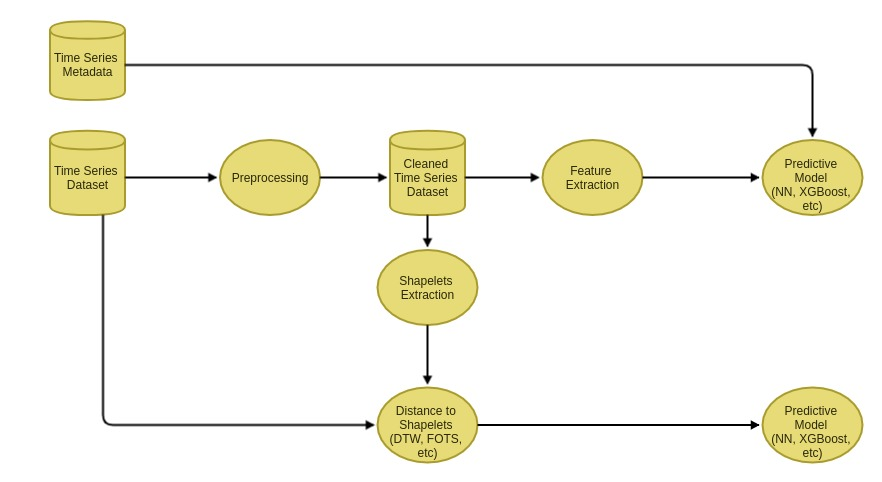
\includegraphics[width=12cm,height=7cm]{report/figures/modeling-schema.jpg}
    \caption{Schéma générale de modélisation}
    \label{fig:modeling_shema}
\end{figure}

\subsection{Modèles basés sur les caractéristiques}\label{sec:feature_based_model}

\subsection{Modèles basés sur les shapelets}\label{sec:shapelet_based_model}
Un Shapelet est défini comme une sous-séquence d'une série temporelle qui est représentative pour la classe \citep{ye2009time}. Ainsi une série temporelle appartient à une classe donnée si elle contient le \textit{shapelet} représentatif de ladite classe. Dans la pratique les séries d'une même classe n'ont pas exactement les mêmes sous-séquences représentatives mais elles ont des sous-séquences qui sont similaires aux sous-séquences représentatives de la classe. 
La classification des séries temporelles peut être réalisée par un arbre de décision (Figure \ref{fig:shapelet_based_dt}) dans lequel l'attribut de division (split) à chaque noeud est un \textit{shapelet} et les données sont séparées en fonction de leur similarité à ce \textit{shapelet}.

\begin{figure}[!h]
    \centering
    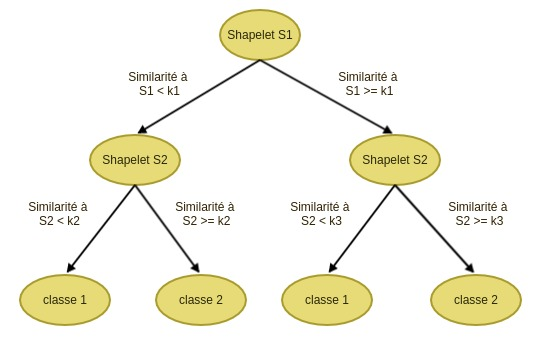
\includegraphics[width=10cm,height=7cm]{report/figures/shapelet-based-tree.jpg}
    \caption{Classification des séries temporelles basée sur les shapelets}
    \label{fig:shapelet_based_dt}
\end{figure}

La classification basées sur les shapelets a trois avantages \citep{ye2009time}:
\begin{itemize}
    \item les résultats sont interprétables 
    \item la robustesse: les shapelets sont des caractéristiques locales des séries temporelles. S'ils sont bien extraits, ils réduisent considérablement le bruit dans les données et rendent ainsi le modèle plus robuste
    \item la rapidité de classification: les shapelets étant des sous-séquences de taille généralement beaucoup plus petite que la taille des séries à classer, il est beaucoup plus rapide de comparer les séries aux shapelets que de comparer les séries entre elles.
\end{itemize}

Pour pourvoir appliquer ce modèle il faut pourvoir extraire les shapelets et définir la notion de similarité entre un shapelet et une série temporelle.

Commençons par donner quelques définitions formelles:

\textbf{Une série temporelle \textit{T}} est une ensemble ordonné de \textit{m} valeurs réelles. $ T = t_1, t_2,...,t_m $. \textit{m} est la taille de la séries.

\textbf{Une sous-série \textit{S} de \textit{T}} est un sous ensemble ordonné de \textit{l} ($ l \leq m $) valeurs de \textit{T}. $ S = T_p, T_{p+1},..., T_{p+l-1}, pour 1 \leq p \leq m-l+1 $. Le nombre de sous-séries peut très rapidement exploser lorsque $l$ est négligeable devant $m$. En effet une série de taille $m$ a exactement $ m-l+1 $ sous-séries de taille $l$. Les données de test de PLASTICC forment un ensemble de $ 3492890 $ de taille $1094$ chacune après qu'on l'imputation des valeurs manquantes. Le nombre de sous-séries possible est donc de $ 3492890 \times (1094 - l + 1)$, un algorithme naif serait donc inutilisable en pratique.

    \textbf{Un Shapelet} est une sous-séries qui permet de séparer l'ensemble des séries temporelles en deux classes suffisamment hétérogènes pour que l'une des classes contienne des séries qui ont une sous-séquence similaire au shapelet tandis que l'autre classe contient des séries qui n'ont pas de sous-séquence similaire au shapelet\cite{fotso2018frobenius}. 

\subsubsection{Mesure de la similarité}
Il existe dans la littérature plusieurs métriques pour mesurer la similarité entre deux séries temporelles de même taille. Nous avons par exemple la distance euclidienne, DTW (Dynamic Time Warping), DUST, PROUD, MUNICH et FOTS \cite{fotso2018frobenius}. Les séries temporelles de PLASTICC étant incertaines, FOTS serait la métrique la plus adaptée car elle est plus robuste à l'incertitude. Cependant, étant contraint par le temps, nous avons utilisé DTW car tslean l'implémente déjà et le calcul des valeurs propres dont a besoin FOTS sur un dataset aussi grand que celui de PLASTICC prendrait beaucoup trop de temps.

La similarité entre une séries $ T $ et une sous-séries $ S $ de taille inférieure ou égales est définie comme la similarité entre $ S $ et la sous-séries de $ T $ de même taille de de $ S $ et la plus similaire à $ S $. 
$$
Sim(S, T) = min \left \{ Sim(S, S'), |S|=|S'| \:  \forall S'\: sous \: séries \: de \: T \right \}
$$

Dans la formule précédente $ Sim $ peut être n'importe qu'elle mesure de similarité entre deux séries temporelles. 

\subsubsection{Extraction des shapelets}
Pour apprende les shapelets nous avons utilisé la bibliothèque tslean\citep{tslearn} qui implémente l'approche proposée par \citet{grabocka2014learning}. Cette approche considère la recherche des shapelets optimaux comme un problème d'optimisation qui débute par un choix aléatoire des shapelets puis les optimise au fur et à mesure en diminuant le taux d'erreur de classification. Le but est de ne pas rechercher dans l'ensemble des candidats possibles car trop grand. tslearn fournit également une heuristique qui permet de déterminer le nombre et la longueur de chacun des shapelets à apprendre. Selon cette heuristique, il nous a fallut apprendre sur les données de plasticc $ 109 $ shapelets de tailles $ 8 $ et $ 218 $ shapelets de tailles $ 7 $. La figure \ref{fig:shapelet_example} donne quelques shapelets que nous avons appris sur plasticc. Les couleurs correspondent aux différents filtres.

\begin{figure}[!h]
    \centering
    \begin{tabular}{c|c}
         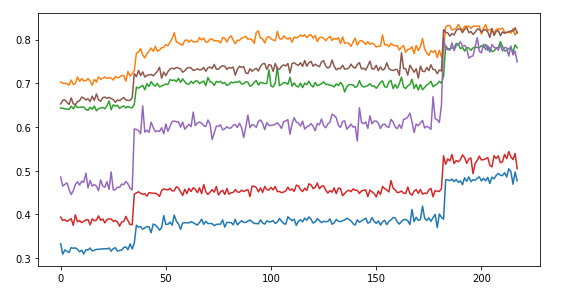
\includegraphics[width=7cm,height=5cm]{report/figures/shapelet.png} & 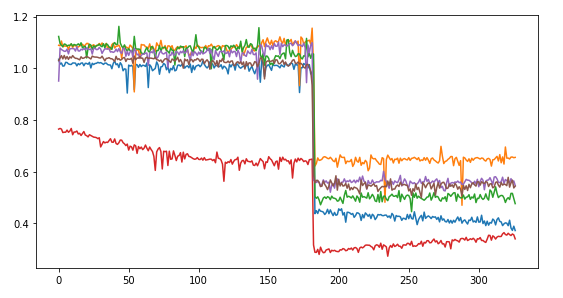
\includegraphics[width=7cm,height=5cm]{report/figures/shapelet2.png}
    \end{tabular}
    \caption{Exemple de shapelets appris sur PLASTICC}
    \label{fig:shapelet_example}
\end{figure}

\section{Évaluation}

\section{Déploiement}